\chapter{Algorytmy detekcji pieszych}
\label{cha:algoDetPiesz}

W~cyfrowej analizie obrazu detekcja pieszych jest jedną z~najbardziej aktywnie rozwijanych dziedzin.
W~ciągu kilkudziesięciu lat powstało ponad tysiąc artykułów poruszających to zagadnienie \cite{zhang2015filtered}, w~których zaproponowano wiele różnych metod.
Większość z~nich opiera się na analizie obrazu tylko w~jednym spektrum: widzialnym albo podczerwieni.
Praca \cite{hwang2015multispectral} pokazała, iż połączenie obu obrazów może dać lepsze wyniki.
Podobnie w~artykule \cite{gonzalez2016pedestrian} wykazano, że analiza multispektralna jest skuteczniejsza w~dzień niż w~nocy (o~około 5\% AMR (ang. \textit{Avrange Miss Rate}).
W~artykule \cite{benenson2014ten} autorzy podsumowują osiągnięcia w~dziedzinie detekcji pieszych w latach 2004 -- 2014.
Wyróżniono ponad 40 różnych podejść do problemu.
Eksperymenty w~artykule są oparte o~bazę danych Caltech-USA, która zawiera obrazy w~kolorze.
Jednym z wniosków jest to, że przez ostanie dziesięć lat największy postęp został osiągnięty głównie dzięki dopracowaniu cech, które są wyodrębniane z obrazu, niż ulepszanie klasyfikatora.
Dodatkowo autorzy połączyli cechy dające najlepsze wyniki i~stworzyli własną metodę, która pozwoliła poprawić o~ok 12\% AMR względem najlepszej badanej wcześniej metody.

Coraz większą popularnością cieszą się rozwiązania oparte o głębokie sieci neuronowe  (DNN ang. \textit{Deep Neural Networks}). W artykule \ref{du2017fused} został zaprezentowany system wykrywania pieszych operaty na fuzji kilkunastu dobrze wyuczonych sieci neuronowych, dając jeden z lepszych wyników detekcji z wykorzystaniem bazy Caltech-USA. 
%ok TODO a coś o głębokich sieciach ? Jakoś pominął Pan ten temat.
%ok TODO 2 jw. ? chociaż jeden przykład - bo to jest teraz na topie....

Dla typowego algorytmu detekcji pieszych można wyróżnić trzy podstawowe etapy:

\section{Ustalenie regionu zainteresowania}

Jest to obszar zwany ROI (ang. \textit{Region Of Interest}), w~którym potencjalnie mogą znajdować się piesi.
Wiele podejść uznaje cały obraz jako ROI i~stosuje okno przesuwne, sprawdzając każdy możliwy fragment obrazu.
Jeżeli scena jest rejestrowana przez nieruchomą kamerę, ROI można określić poprzez różnicę między zapamiętanym tłem a~aktualnym obrazem (tzn. modelowanie i~odejmowanie tła). 
Analiza przepływu optycznego również pozwala na wyodrębnienie obszaru, w~których obserwowany jest ruch inny niż na pozostałej części sceny. 
Inną metodą jest zastosowanie słabszego, bardziej ogólnego, ale mniej wymagającego obliczeniowo  klasyfikatora.
Wyodrębnienie ROI jest bardzo istotne w~przypadku pracy w~czasie rzeczywistym, ze względu na ograniczony maksymalny czas analizy pojedynczego obrazu.

\section{Wyodrębnienie cech}

Do najbardziej popularnych cech można zaliczyć:

\begin{enumerate}
\item Histogramy zorientowanych gradientów (HOG ang. \textit{Histogram of Oriented Gradients }).
Algorytm został zaproponowany przez N.Dalala i B. Triggsa w~pracy \cite{dalal2005histograms} i~stał się jedną z~najbardziej popularnych metod w~dziedzinie detekcji ludzi. 
Jest cały czas rozwijany i~modyfikowany w~wielu pracach naukowych.
W pierwszej kolejności zostają obliczone gradienty dla obrazu, za pomocą dwóch masek kierunkowych [-1 0 1] i [-1 0 1]$^T$. Gradienty mogą być ze znakiem lub bez. Na rysunku \ref{fig:hog} przedstawiono przykład uzyskiwania gradientów. Następnie tworzone są histogramy orientacji na podstawie gradientów uzyskanych z pkt. 1. Histogram ma z~góry zadaną liczbę przedziałów i zawiera dane z komórki (ang. \textit{cell}) o określonej wielkości (np. kwadrat 6x6). Wagi orientacji poszczególnych pikseli wynikają z wartości wypadkowej gradientu. Na rysunku \ref{fig:hog2} zaprezentowano przykładowe histogramy.
Komórki łączone są w bloki, w obrębie których następuje normalizacja. Ma ona na celu wyrównanie kontrastów pomiędzy sąsiadującymi blokami komórek. Bloki mają z góry ustalony rozmiar i nakładają się na siebie.Połączenie wszystkich histogramów we wszystkich blokach w jeden wektor cech.

\begin{figure}
\centering
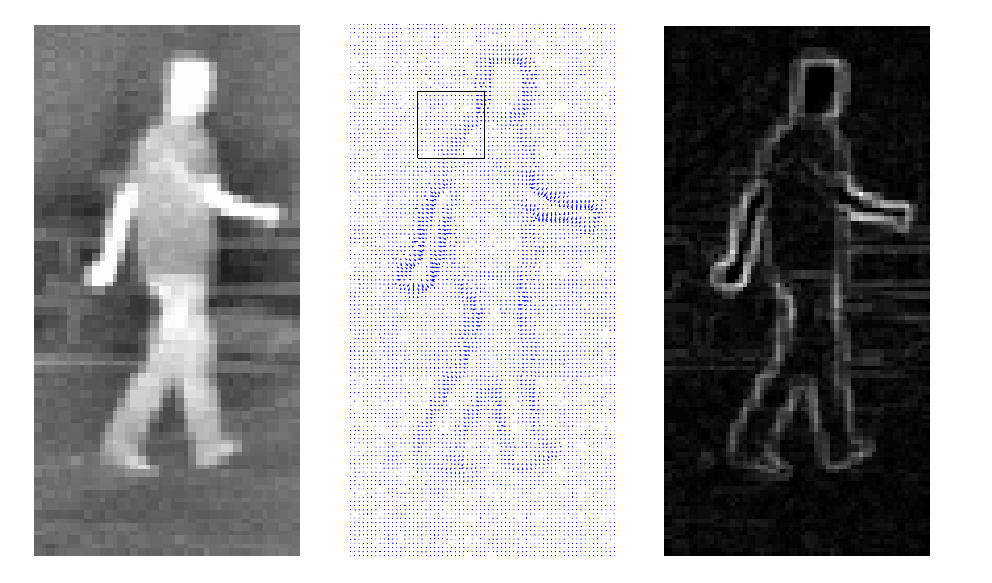
\includegraphics[width=0.5\linewidth]{images/hog}
\caption[Obliczanie gradientów dla obrazu.]{Obliczanie gradientów dla obrazu. Po lewej oryginalny obraz, pośrodku kierunki gradientów, po prawej wartości modułów \cite{suard2006pedestrian}.}
\label{fig:hog}
\end{figure}

\begin{figure}
\centering
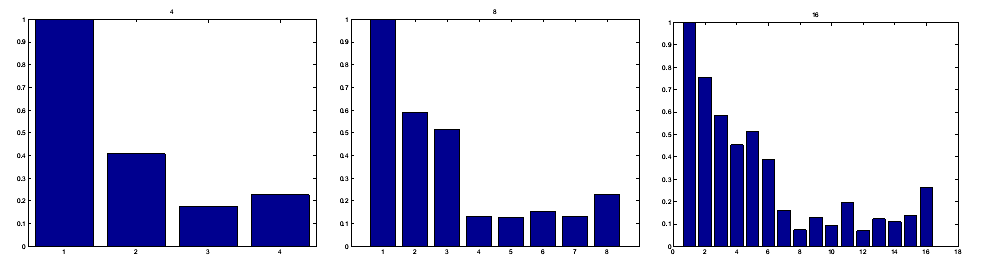
\includegraphics[width=0.7\linewidth]{images/hog2}
\caption[Przykładowe histogramy]{Przykłady histogramów o różnej ilości przedziałów \cite{suard2006pedestrian}.}
\label{fig:hog2}
\end{figure}

%TT w dalszym rozdziale jest to szczegółowo opsane.
%TODO 2 Skoro tak to proszę dać więcej szczegółów 

\item Lokalne wzorce binarne LBP (ang. \textit{Local Binary Paterns}).
Oryginalnie deskryptory te zostały zaproponowane  do opisu tekstur \cite{ojala2002multiresolution}. %OK TODO \cite też coś ojala - 2 tego Pan nie zrobił.
Analizowany obraz zostaje podzielony na bloki.
Następnie, do każdego piksela w~bloku zostaje przypisany wzorzec binarny na podstawie wartości pikseli w~jego sąsiedztwie.
Jeżeli wartość sąsiadującego piksela jest większa od centralnego, to przyjmuje on wartość~1. 
W~ten sposób do każdego piksela przypisywany jest wzorzec binarny (np. 1100110). %OK TODO 2 7 bitów.. raczej 8
Następnie zostaje obliczony histogram wzorców dla każdego bloku.
Histogramy z wszystkich bloków wchodzących w~skład obrazu (okna detekcji) tworzą wektor cech.

\item Falki Haara.
Określają różnicę w~kontraście między dwoma przylegającymi prostokątnymi obszarami. 
W~oryginalnej pracy P.Viola i M.Jones z~2001 \cite{viola2001rapid} autorzy rozważali 3 rodzaje cech: 
\begin{itemize}
	\item dwa obszary mające ten sam rozmiar i~kształt oraz przylegające do siebie horyzontalnie bądź wertykalnie, gdzie cechę stanowi różnica sumy pikseli zawartych w~każdym z regionów ( Układ A i B na rysunku \ref(fig:haar)), 
	\item obszar składający się z 3 prostokątów przylegających do siebie, gdzie od sumy środkowego elementu jest odejmowana suma dwóch zewnętrznych (układ C),
	\item układ 4 prostokątów, gdzie suma jest różnicą między obszarami po przekątnej (układ D). %TODO 2 niejasne...
\end{itemize}

\begin{figure}
\centering
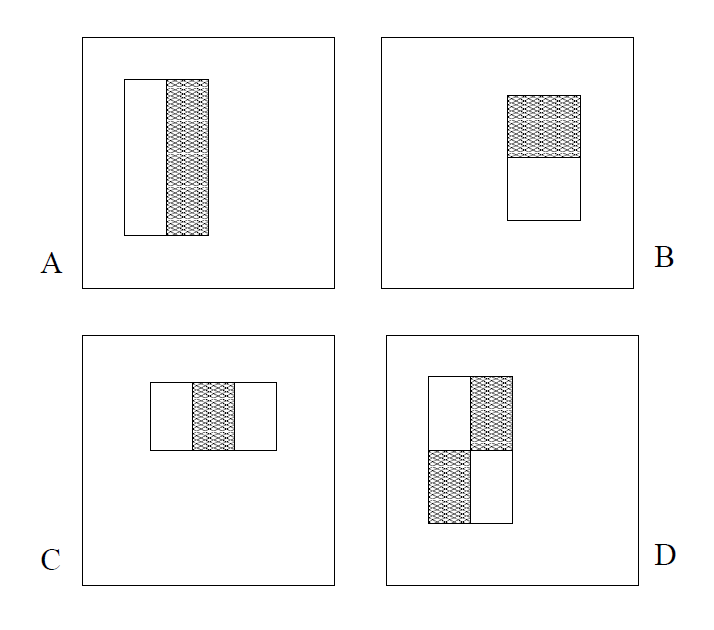
\includegraphics[width=0.5\linewidth]{images/haar}
\caption[Falki Harrra.]{Przykładowe prostokąty służące do określenia cech. Od sumy pikseli zawartych w~białym prostokącie zostaje odjęta suma pikseli w~szarym. \cite{viola2001rapid}.}
\label{fig:haar}
\end{figure}
%OK TODO 2 obrazek by bardzo pomógł
Cechy są łatwe do skalowania i~nie wymagają dużych nakładów obliczeniowych. W celu szybkiego obliczania tych cech stosuje się tzw. \textit{intergral image}. Dla każdego puntu o~współrzędnych x,y zostaje obliczona suma wartości pikseli znajdujących się na lewo i~nad od lokacji~x,y. Dzięki temu, aby obliczyć sumę pikseli w~danym kwadracie wystarczą jedynie cztery punkty referencyjne. Na przykład, by obliczyć sumę pikseli w~prostokącie D na rysunku \ref{fig:integralImage} wystarczy rozwiązać równanie $D = 4 + 1 -(2 + 3)$.

\begin{figure}
\centering
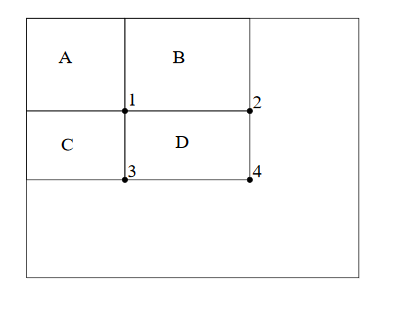
\includegraphics[width=0.5\linewidth]{images/integralImage}
\caption[IntegralImage.]{Obliczanie sumy pikseli za pomocą \textit{integral image}.  \cite{viola2001rapid}.}
\label{fig:integralImage}
\end{figure}
%OK TODO 2 można Pan dodać, że ich do ich obliczania można wykorzystać tzw. intergral image.

\item Kolor. 
W~analizie obrazów wykorzystuje różne przestrzenie barw np. RGB, HSV oraz LUV. 
Głównie wtedy, gdy kolor wykrywanego obiektu jest kluczowy (np. znaki drogowe, światła na skrzyżowaniu). 
Jako cechę można go wykorzystać w~kilku formach. 
Momenty koloru (ang. \textit{Color Moments}) jest to średnia, wariancja i~odchylenie standardowe występowania danego koloru na obrazie. 
Histogram określa częstość występowania danego koloru, a~wektor koherencji koloru (CCV ang. \textit{Color Coherence Vectors}) określa w~jakim stopniu piksele danego koloru są częścią obszaru o~podobnym kolorze (np. obraz zielonej łąki na którym pasie się jedna fioletowa krowa. Kolor zielony na obrazie byłby rozłożony równomiernie natomiast fioletowy byłby skupiony w~pojedynczym rejonie koherencji -- krowy) \cite{kodituwakku2004comparison}.

\end{enumerate}

\section{Klasyfikator}

Otrzymany wektor cech jest następnie poddany klasyfikacji, której wynik decyduje czy obraz zawiera człowieka.
W pracy \cite{benenson2014ten} autorzy wyróżnili 3 dominujące rodziny metod:

\begin{enumerate}
\item Rodzina DPM (ang. \textit{Deformable Part Model})
%
Technika zakłada, że obiekty mogą być zamodelowane poprzez części ułożone w~deformowanych konfiguracjach. 
Model składa się z~głównego, globalnego filtra, który stanowi punkt odniesienia dla pozostałych części. 
Każda część zawiera swój własny filtr wraz z~zestawem dozwolonych pozycji względem okna detekcyjnego oraz koszt deformacji dla każdej z tych pozycji. 
Suma wyniku uzyskanego z~filtra głównego wraz z~jego częściami stanowi o~wyniku detekcji \cite{felzenszwalb2008discriminatively}.

\item Deep networks.
%OK TODO 2 1. Musi Pan wraznie zaznaczyć, że to jest nieco odrebne, w sensie ze to jest ekstrakca + klasyfikacja.
%OK TODO 2 2. Jakiś rysunek by też pomógł.

\begin{figure}
\centering
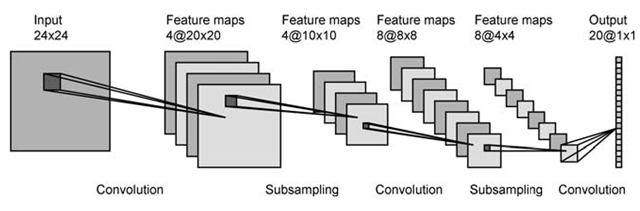
\includegraphics[width=0.5\linewidth]{images/DNN}
\caption[IntegralImage.]{Schemat przykładowej sieci konwolucyjnej.}
\label{fig:DNN}
\end{figure}

Głębokie sieci neuronowe posiadają kilkanaście warstw ukrytych między warstwą wejściową i wyjściową. 
Ich działanie polega na tym, że po podaniu wektora cech na warstwę wejściową wytrenowanej sieci, w~warstwie wyjściowej aktywuje się neutron odpowiedzialny za detekcję danej klasy. 
W~analizie obrazu szczególnie chętnie wykorzystywane są sieci konwolucyjne. W odróżnieniu od klasycznego podejścia głębokie sieci konwolucyjne łączą w sobie oba zadania: wyodrębnianie cech i klasyfikacje.
Neurony pierwszej warstwy ukrytej są podłączone jedynie do wybranego fragmentu warstwy wejściowej (np. okna 24x24). %OK TODO 2 ten histogram jest dla mnie niejasny %To usunę 
Jest to tzw. warstwa konwolucyjna. 
Neurony w~tej warstwie dzielą wspólne wagi dla swoich wejść i bias. 
Sieć posiada zazwyczaj kilkanaście takich warstw -- każda wykrywająca pojedynczą cechę. 
Pozwala to na redukcję liczby neutronów i~parametrów potrzebnych do uzyskania w procesie uczenia. 
Do warstw konwlucyjnych dochodzą warstwy sumujące (ang. \textit{Polling Layers}). 
Ich zadaniem jest generalizacja informacji z poprzedniej warstwy. 
Sieć zamyka w pełni połączona z poprzednią, warstwa wyjściowa. Na rysunku \ref{fig:DNN} przedstawiono schemat przykładowej sieci konwolucyjnej.
%OK TODO 2 to ostatnie zdanie do uzupełnienia - niejasne.

\item Decision forests

Lasy decyzyjne to zbiory nieskorelowanych drzew decyzyjnych. 
Pojedyncze drzewo jest graficznym odwzorowaniem procesu decyzyjnego. 
Algorytm uczenia drzew wykorzystuje przykłady (wektor cech) i związane z nimi konsekwencje (klasyfikacja obiektu).

%TODO 2 też może rysunek

\item inne: np. SVM (ang. Support Vector Machine -- maszyna wektorów nośnych), AdaBoost itp.


\end{enumerate}

%TODO Nie omówił Pan specyfiki detekcji w podczerwieni.
%TODO 2 Czy specyfika detekcji w podczerwieni gdzies jest ?

